\documentclass[11pt]{article}
\usepackage[left=25mm, right=25mm, top=25mm, bottom=25mm, includehead=true, includefoot=true]{geometry}

\usepackage{graphicx}
\usepackage{url}
\usepackage{natbib} % For referencing
\usepackage{authblk} % For author lists
\usepackage[parfill]{parskip} % Line between paragraphs

\pagenumbering{gobble} % Turn off page numbers

% Make all headings the same size (11pt):
\usepackage{sectsty}
\sectionfont{\normalsize}
\subsectionfont{\normalsize}
\subsubsectionfont{\normalsize}
\paragraphfont{\normalsize}


\renewcommand{\abstractname}{Summary} % Make 'abstract' be called 'Summary'


% This makes links and bookmarks in the pdf output (should be last usepackage command because it overrides lots of other commands)
\usepackage[pdftex]{hyperref} 
\hypersetup{pdfborder={0 0 0} } % This turns off the stupid colourful border around links



% **************  TITLE AND AUTHOR INFORMATION **************

\title{The Title of the Paper}

\author[1]{Author A\thanks{author.a@university.edu}}
\author[1]{Author B\thanks{author.b@university.edu}}
\author[2]{Author C\thanks{author.c@university.edu}}
\affil[1]{Department of Computer Science, \LaTeX\ University}
\affil[2]{Department of Mechanical Engineering, \LaTeX\ University}

\renewcommand\Authands{ and } % correct last comma in author list

\begin{document}

\maketitle

% **************  ABSTRACT/SUMMARY  **************

\begin{abstract}
\centering

Summary of no more than 100 words \textit{(this needs to be pasted into the `Abstract� box on EasyChair)}.

$ $ \\ {\bf KEYWORDS:} 5 keywords or short phrases relevant to the work \textit{(these need to be pasted into the `Keywords� box on EasyChair)}.

\end{abstract}

% **************  MAIN BODY OF THE PAPER **************

\section{Introduction to guidelines}

The purpose of providing these notes is to standardise the format of the short papers submitted to GISRUK 2015. These notes are based on author guidelines previously produced for the GISRUK conference series which in turn were based on other guidelines.

The pages should have margins of 2.5 cm all round. The base font should be Times New Roman 11pt, or closest equivalent and text should be single spaced. Each section of the paper should be numbered. Section headings should be left-justified and given in bold type.  A slightly larger font should be used for the title of the paper and the authors (16pt and 14pt respectively). The first line of each paragraph in each section should \textbf{NOT} be indented.

\subsection{Sub-sections}

Sub-sections should also be numbered as shown here. The sub-section heading should be left-justified and given in bold type (11pt). 

\section{Figures, Tables and Equations,}

Tables should be as shown below (or as close as possible) and should be referenced as Table~\ref{first_table} in the text.

\begin{table}[htdp]
\caption{GISRUK Conferences}
\begin{center}
\begin{tabular}{c|c}
\hline 
Year	 & City \\
\hline 
2007 & Maynooth \\
2008 & Manchester \\
2009 & Durham \\
2010 & UCL \\
2011 & Portsmouth \\
2012 & Lancaster\\ 
\hline
\end{tabular}
\end{center}
\label{first_table}
\end{table}%

Equations should be centred on the page and numbered consecutively in the right-hand margin, as below. They should be referred to in the text as Equation~\ref{first_equation}. 

\begin{equation}
E=mc^2
\label{first_equation}
\end{equation}

Figures should be presented as an integral part of the paper and should be referred to as Figure~\ref{first_figure} in the text.

\begin{figure}[htbp] \begin{center} 
\resizebox{0.3\textwidth}{!}{ 
	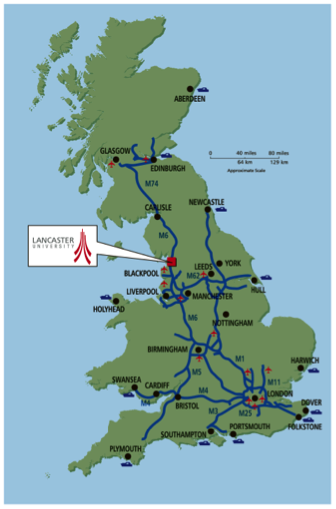
\includegraphics{lancaster.png}
} \caption{Location of Lancaster University} \label{first_figure} \end{center} \end{figure} %


\section{References and Citations}

A list of references cited should be provided at the end of the paper using the Harvard format as shown below. Citations of these within the text should be given as follows: papers such as an interesting one by \citet{HARVEY:2006} and also interesting books \citep{DAY:2006}.

\section{File format}

Papers should be submitted in unrestricted \textbf{pdf} format. Authors are requested to keep to the word limit of 1500 words. 

\section{Acknowledgements}

Acknowledgement should be made of any funding bodies who have supported the work reported in the paper, of those who have given permission for their work to be reproduced or of individuals whose particular assistance is due recognition. Acknowledge data providers here where appropriate.

\section{Biography}
All contributing authors should include a biography of no more than 50 words each outlining their career stage and research interests.


% **************  REFERENCES **************

\bibliographystyle{apa}
\bibliography{references.bib}

\end{document}
